\chapter{Funcionamiento del programa}

\subsection*{Restricciones de ejecución}

\subsection*{Banderas de entrada}


\chapter{Conjunto de 9 proteínas}

	\begin{figure}[H]
	\subsection*{IdPDB:1a2b}	
	\hspace{-0.3cm} 
	\begin{subfigure}{0.49\textwidth}
		\centering
		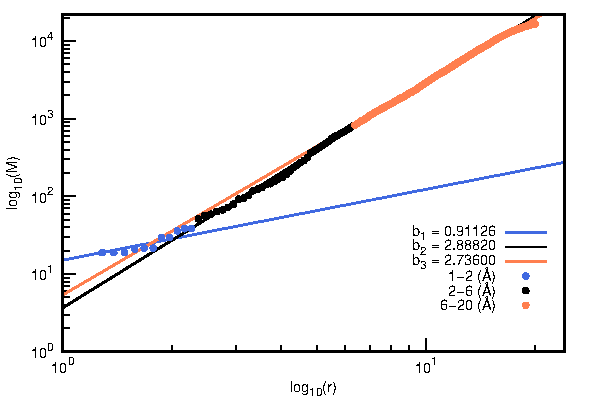
\includegraphics[width=\linewidth,page=1]{graphs/PDBs/1a2b/1a2baddH.pdf}
		\caption{(1)}
	\end{subfigure}
	\hspace{0.2cm}
	\begin{subfigure}{0.49\textwidth}
		\centering
		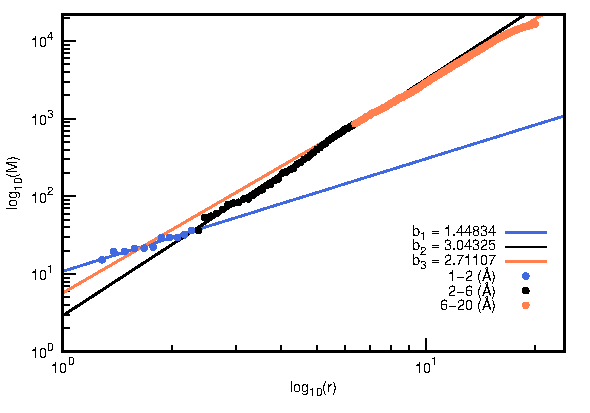
\includegraphics[width=\linewidth,page=1]{graphs/PDBs/1a2b/1a2bEm.pdf}
		\caption{(2)}
	\end{subfigure}
	
	\vspace{0cm} % Espacio entre filas
	
	\hspace{-0.3cm} 
	\begin{subfigure}{0.49\textwidth}
		\centering
		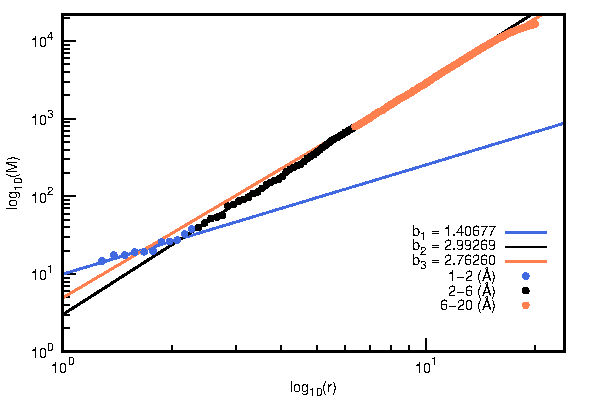
\includegraphics[width=\linewidth,page=1]{graphs/PDBs/1a2b/1a2bEq.pdf}
		\caption{(3)}
	\end{subfigure}
	\hspace{0.2cm}
	\begin{subfigure}{0.49\textwidth} % M\'{a}s ancho para centrar
		\centering
		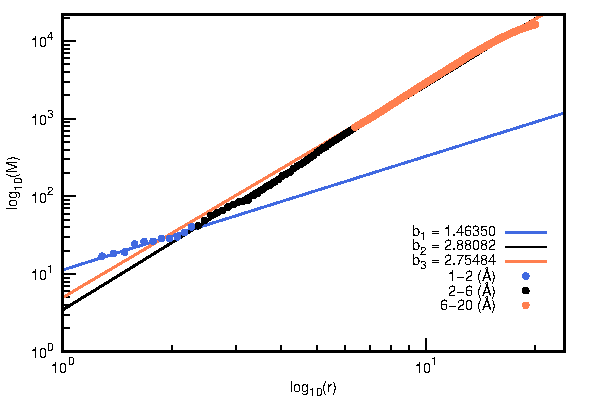
\includegraphics[width=\linewidth,page=1]{graphs/PDBs/1a2b/1a2b1ns.pdf}
		\caption{(4)}
	\end{subfigure}
	
	\caption{
		Regresiones lineales de $log_{10}r$ vs $log_{10}M(r)$ correspondiente a cuatro etapas de procesamiento de la primera prote\'{i}na con \textit{IdPDB:1a2b} de la Tabla \ref{Tabla:ids9}: (1) Adici\'{o}n de \'{a}tomos de hidr\'{o}geno al sistema proteico; (2) al minimizar la energ\'{i´}a de la estructura molecular; (3) equilibrando el sistema bajo condiciones termodin\'{a}micas controladas; y (4) despu\'{e}s de una din\'{a}mica molecular de 1 ns.}
	\label{fig:1a2b}
\end{figure}

\begin{figure}[H]
	\subsection*{IdPDB:1a3n}
	
	\hspace{-0.3cm} 
	\begin{subfigure}{0.49\textwidth}
		\centering
		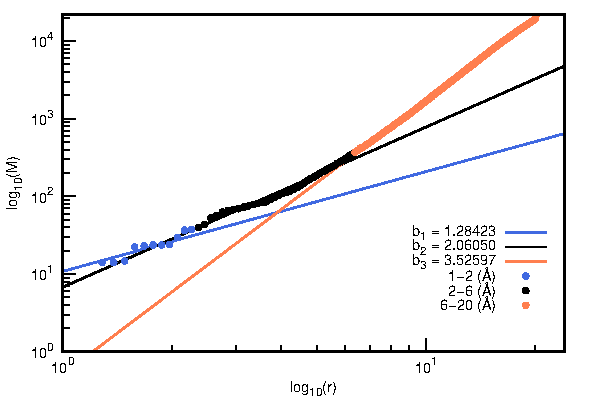
\includegraphics[width=\linewidth,page=1]{graphs/PDBs/1a3n/1a3naddH.pdf}
		\caption{(1)}
	\end{subfigure}
	\hspace{0.2cm}
	\begin{subfigure}{0.49\textwidth}
		\centering
		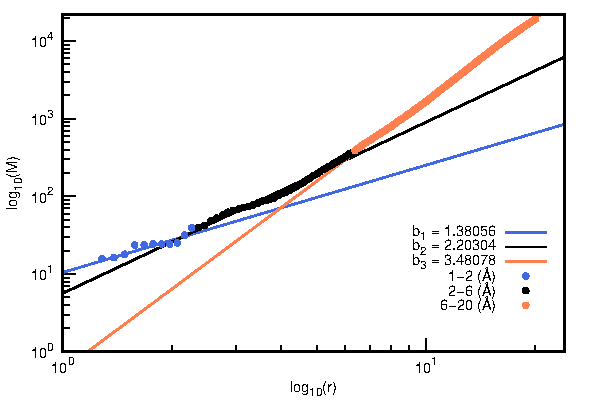
\includegraphics[width=\linewidth,page=1]{graphs/PDBs/1a3n/1a3nEm.pdf}
		\caption{(2)}
	\end{subfigure}
	
	\vspace{0cm} % Espacio entre filas
	
	\hspace{-0.3cm} 
	\begin{subfigure}{0.49\textwidth}
		\centering
		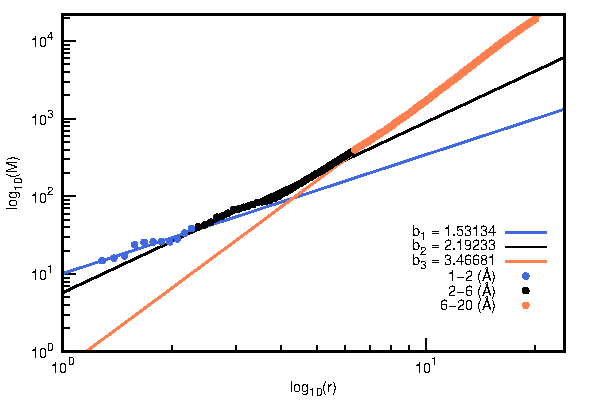
\includegraphics[width=\linewidth,page=1]{graphs/PDBs/1a3n/1a3nEq.pdf}
		\caption{(3)}
	\end{subfigure}
	\hspace{0.2cm}
	\begin{subfigure}{0.49\textwidth} % M\'{a}s ancho para centrar
		\centering
		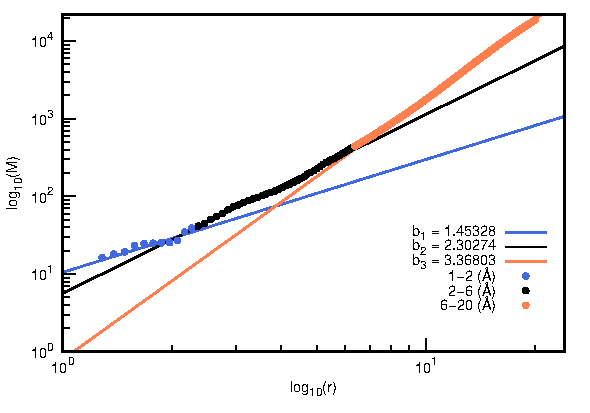
\includegraphics[width=\linewidth,page=1]{graphs/PDBs/1a3n/1a3n1ns.pdf}
		\caption{(4)}
	\end{subfigure}
	\caption{Regresiones lineales de $log_{10}r$ vs $log_{10}M(r)$ correspondiente a cuatro etapas de procesamiento de la segunda prote\'{i}na con \textit{IdPDB:1a3n} de la Tabla \ref{Tabla:ids9}: (1) Adici\'{o}n de \'{a}tomos de hidr\'{o}geno al sistema proteico; (2) al minimizar la energ\'{i´}a de la estructura molecular; (3) equilibrando el sistema bajo condiciones termodin\'{a}micas controladas; y (4) despu\'{e}s de una din\'{a}mica molecular de 1 ns.}
	\label{fig:1a3n}
\end{figure}

\begin{figure}[H]
	\subsection*{IdPDB:1a8m}
	
	\hspace{-0.3cm} 
	\begin{subfigure}{0.49\textwidth}
		\centering
		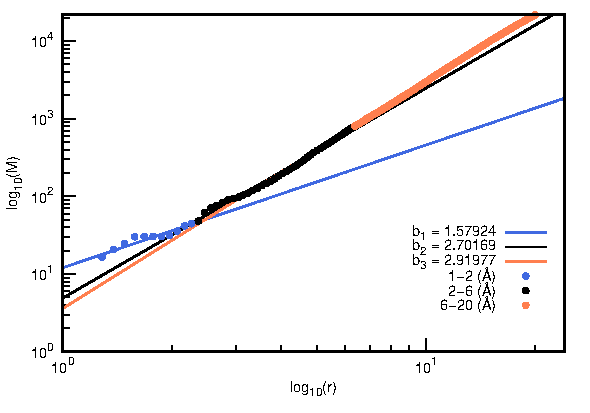
\includegraphics[width=\linewidth,page=1]{graphs/PDBs/1a8m/1a8maddH.pdf}
		\caption{(1)}
	\end{subfigure}
	\hspace{0.2cm}
	\begin{subfigure}{0.49\textwidth}
		\centering
		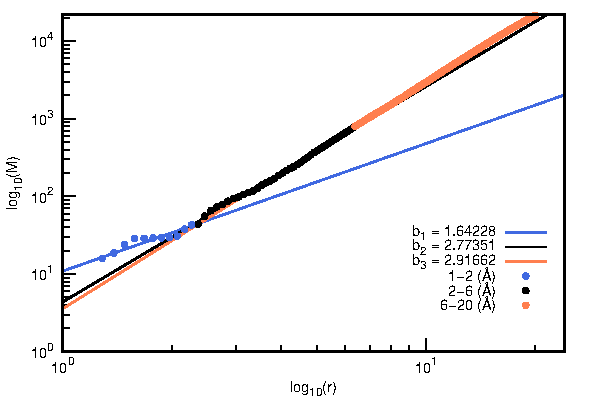
\includegraphics[width=\linewidth,page=1]{graphs/PDBs/1a8m/1a8mEm.pdf}
		\caption{(2)}
	\end{subfigure}
	
	\vspace{0cm} % Espacio entre filas
	
	\hspace{-0.3cm} 
	\begin{subfigure}{0.49\textwidth}
		\centering
		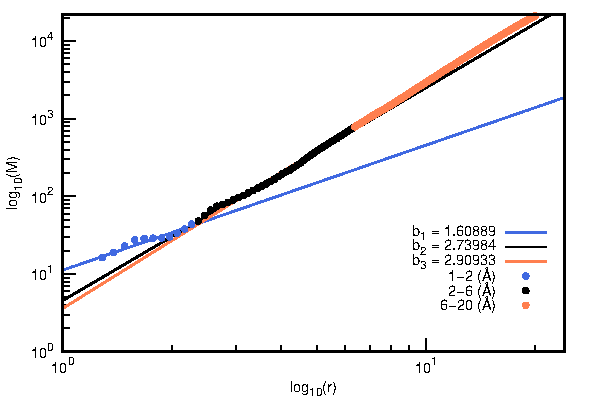
\includegraphics[width=\linewidth,page=1]{graphs/PDBs/1a8m/1a8mEq.pdf}
		\caption{(3)}
	\end{subfigure}
	\hspace{0.2cm}
	\begin{subfigure}{0.49\textwidth} % M\'{a}s ancho para centrar
		\centering
		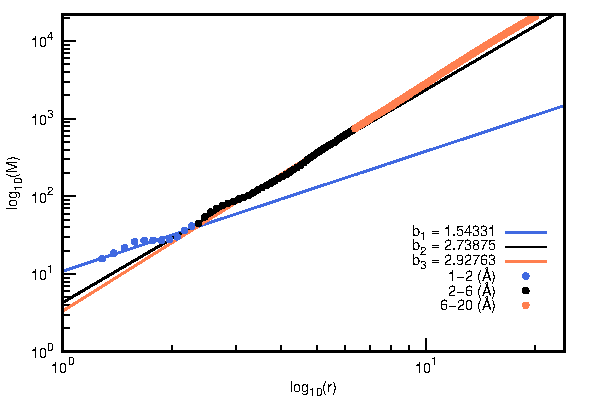
\includegraphics[width=\linewidth,page=1]{graphs/PDBs/1a8m/1a8m1ns.pdf}
		\caption{(4)}
	\end{subfigure}
	\caption{Regresiones lineales de $log_{10}r$ vs $log_{10}M(r)$ correspondiente a cuatro etapas de procesamiento de la cuarta prote\'{i}na con \textit{IdPDB:1a8m} de la Tabla \ref{Tabla:ids9}: (1) Adici\'{o}n de \'{a}tomos de hidr\'{o}geno al sistema proteico; (2) al minimizar la energ\'{i´}a de la estructura molecular; (3) equilibrando el sistema bajo condiciones termodin\'{a}micas controladas; y (4) despu\'{e}s de una din\'{a}mica molecular de 1 ns.}
	\label{fig:1a8m}
\end{figure}


\begin{figure}[H]
	\subsection*{IdPDB:1a9w}
	
	\hspace{-0.3cm} 
	\begin{subfigure}{0.49\textwidth}
		\centering
		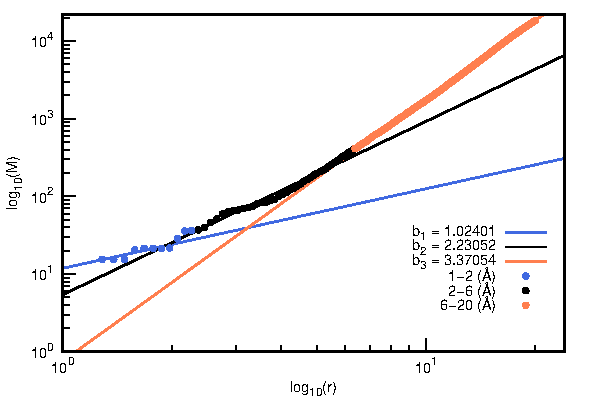
\includegraphics[width=\linewidth,page=1]{graphs/PDBs/1a9w/1a9waddH.pdf}
		\caption{(1)}
	\end{subfigure}
	\hspace{0.2cm}
	\begin{subfigure}{0.49\textwidth}
		\centering
		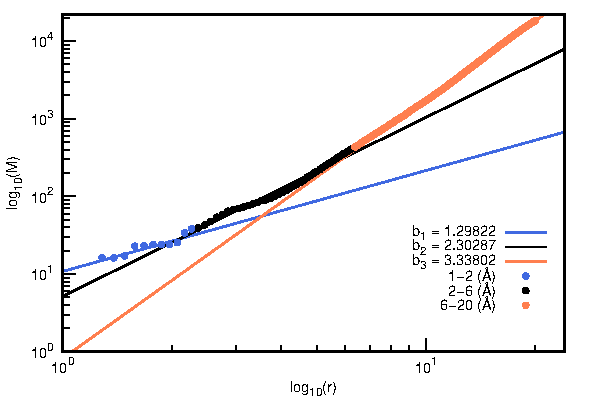
\includegraphics[width=\linewidth,page=1]{graphs/PDBs/1a9w/1a9wEm.pdf}
		\caption{(2)}
	\end{subfigure}
	
	\vspace{0cm} % Espacio entre filas
	
	\hspace{-0.3cm} 
	\begin{subfigure}{0.49\textwidth}
		\centering
		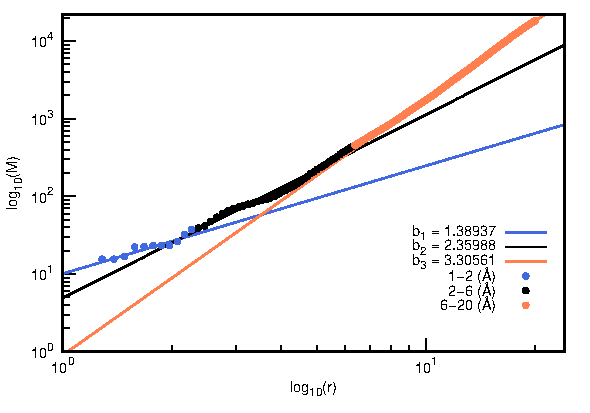
\includegraphics[width=\linewidth,page=1]{graphs/PDBs/1a9w/1a9wEq.pdf}
		\caption{(3)}
	\end{subfigure}
	\hspace{0.2cm}
	\begin{subfigure}{0.49\textwidth} % M\'{a}s ancho para centrar
		\centering
		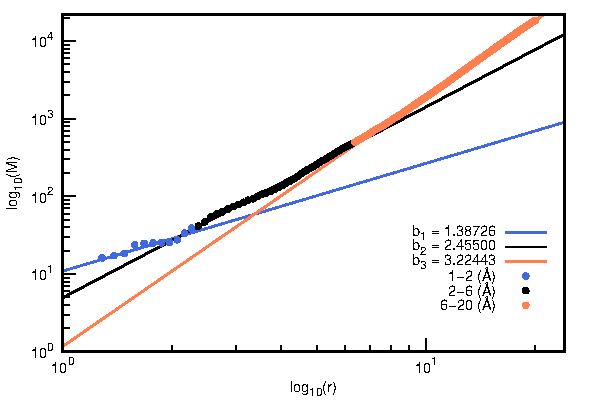
\includegraphics[width=\linewidth,page=1]{graphs/PDBs/1a9w/1a9w1ns.pdf}
		\caption{(4)}
	\end{subfigure}
	\caption{Regresiones lineales de $log_{10}r$ vs $log_{10}M(r)$ correspondiente a cuatro etapas de procesamiento de la quinta prote\'{i}na con \textit{IdPDB:1a9w} de la Tabla \ref{Tabla:ids9}: (1) Adici\'{o}n de \'{a}tomos de hidr\'{o}geno al sistema proteico; (2) al minimizar la energ\'{i´}a de la estructura molecular; (3) equilibrando el sistema bajo condiciones termodin\'{a}micas controladas; y (4) despu\'{e}s de una din\'{a}mica molecular de 1 ns.}
	\label{fig:1a9w}
\end{figure}

\begin{figure}[H]
	\subsection*{IdPDB:1a52}
	
	\hspace{-0.3cm} 
	\begin{subfigure}{0.49\textwidth}
		\centering
		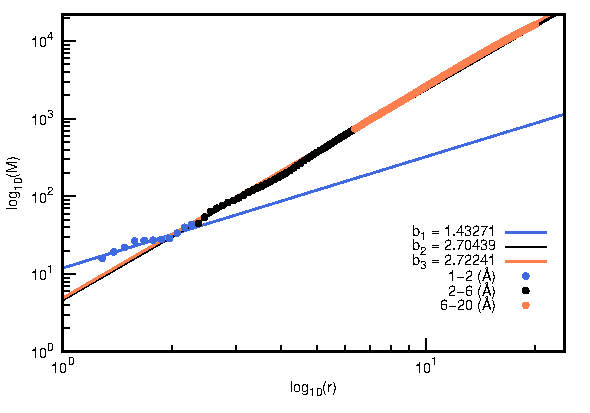
\includegraphics[width=\linewidth,page=1]{graphs/PDBs/1a52/1a52addH.pdf}
		\caption{(1)}
	\end{subfigure}
	\hspace{0.2cm}
	\begin{subfigure}{0.49\textwidth}
		\centering
		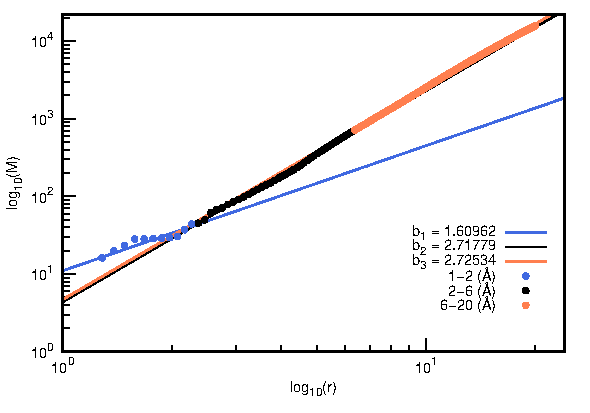
\includegraphics[width=\linewidth,page=1]{graphs/PDBs/1a52/1a52Em.pdf}
		\caption{(2)}
	\end{subfigure}
	
	\vspace{0cm} % Espacio entre filas
	
	\hspace{-0.3cm} 
	\begin{subfigure}{0.49\textwidth}
		\centering
		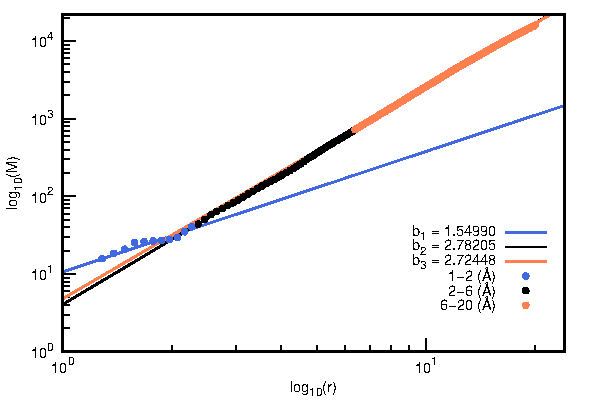
\includegraphics[width=\linewidth,page=1]{graphs/PDBs/1a52/1a52Eq.pdf}
		\caption{(3)}
	\end{subfigure}
	\hspace{0.2cm}
	\begin{subfigure}{0.49\textwidth} % M\'{a}s ancho para centrar
		\centering
		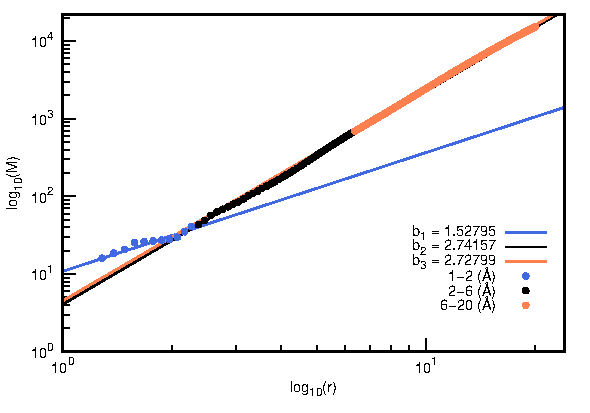
\includegraphics[width=\linewidth,page=1]{graphs/PDBs/1a52/1a521ns.pdf}
		\caption{(4)}
	\end{subfigure}
	\caption{Regresiones lineales de $log_{10}r$ vs $log_{10}M(r)$ correspondiente a cuatro etapas de procesamiento de la tercera prote\'{i}na con \textit{IdPDB:1a52} de la Tabla \ref{Tabla:ids9}: (1) Adici\'{o}n de \'{a}tomos de hidr\'{o}geno al sistema proteico; (2) al minimizar la energ\'{i´}a de la estructura molecular; (3) equilibrando el sistema bajo condiciones termodin\'{a}micas controladas; y (4) despu\'{e}s de una din\'{a}mica molecular de 1 ns.}
	\label{fig:1a52}
\end{figure}


\begin{figure}[H]
	\subsection*{IdPDB:1auk}
	\hspace{-0.3cm} 
	\begin{subfigure}{0.49\textwidth}
		\centering
		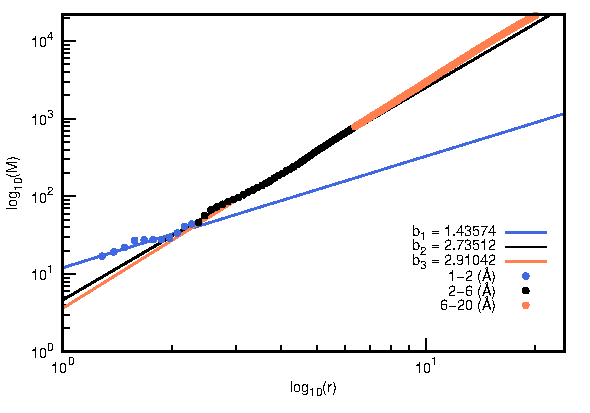
\includegraphics[width=\linewidth,page=1]{graphs/PDBs/1auk/1aukaddH.pdf}
		\caption{(1)}
	\end{subfigure}
	\hspace{0.2cm}
	\begin{subfigure}{0.49\textwidth}
		\centering
		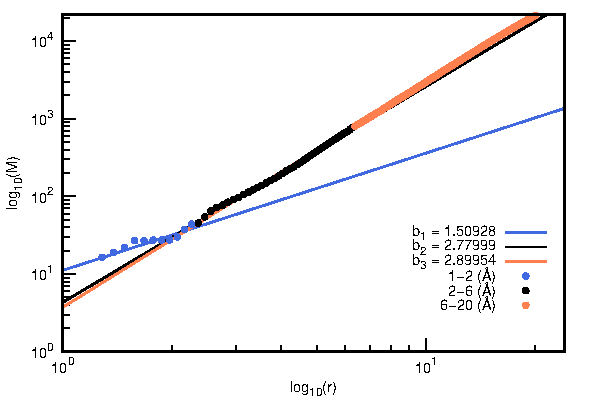
\includegraphics[width=\linewidth,page=1]{graphs/PDBs/1auk/1aukEm.pdf}
		\caption{(2)}
	\end{subfigure}
	
	\vspace{0cm} % Espacio entre filas
	
	\hspace{-0.3cm} 
	\begin{subfigure}{0.49\textwidth}
		\centering
		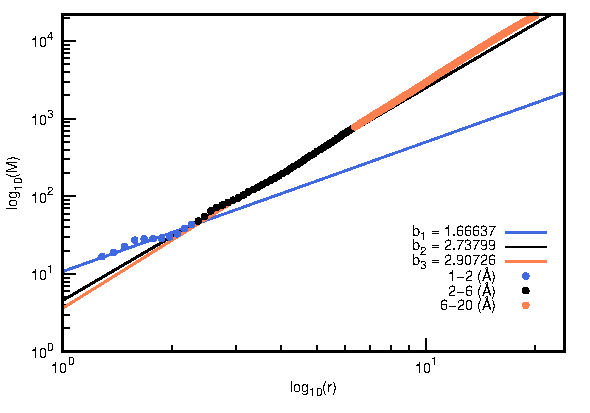
\includegraphics[width=\linewidth,page=1]{graphs/PDBs/1auk/1aukEq.pdf}
		\caption{(3)}
	\end{subfigure}
	\hspace{0.2cm}
	\begin{subfigure}{0.49\textwidth} % M\'{a}s ancho para centrar
		\centering
		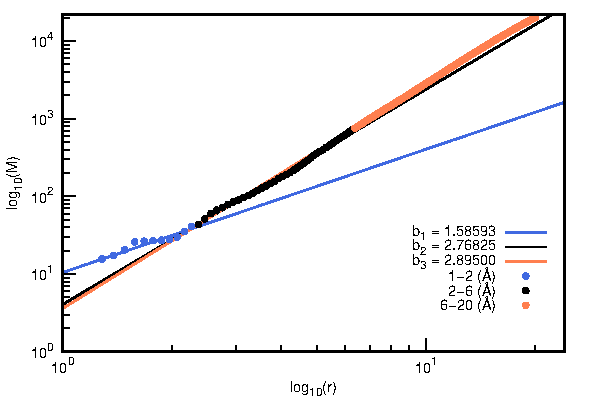
\includegraphics[width=\linewidth,page=1]{graphs/PDBs/1auk/1auk1ns.pdf}
		\caption{(4)}
	\end{subfigure}
	\caption{Regresiones lineales de $log_{10}r$ vs $log_{10}M(r)$ correspondiente a cuatro etapas de procesamiento de la sexta prote\'{i}na con \textit{IdPDB:1auk} de la Tabla \ref{Tabla:ids9}: (1) Adici\'{o}n de \'{a}tomos de hidr\'{o}geno al sistema proteico; (2) al minimizar la energ\'{i´}a de la estructura molecular; (3) equilibrando el sistema bajo condiciones termodin\'{a}micas controladas; y (4) despu\'{e}s de una din\'{a}mica molecular de 1 ns.}
	\label{fig:1auk}
\end{figure}

\begin{figure}[H]
	\subsection*{IdPDB:1b3e}
	
	\hspace{-0.3cm} 
	\begin{subfigure}{0.49\textwidth}
		\centering
		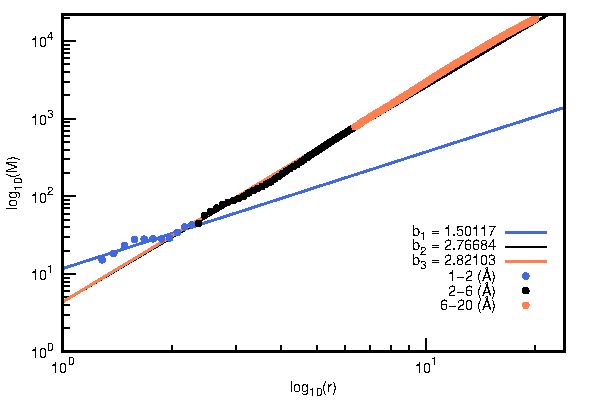
\includegraphics[width=\linewidth,page=1]{graphs/PDBs/1b3e/1b3eaddH.pdf}
		\caption{(1)}
	\end{subfigure}
	\hspace{0.2cm}
	\begin{subfigure}{0.49\textwidth}
		\centering
		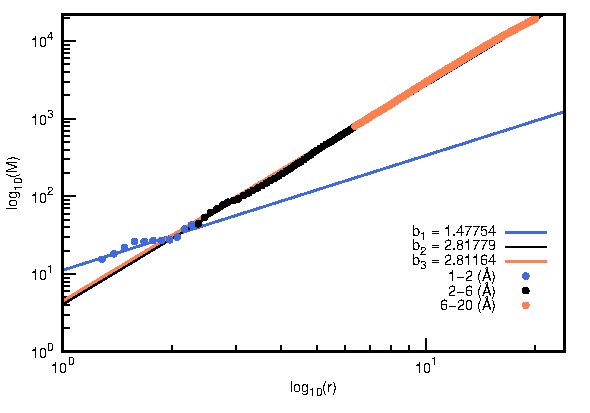
\includegraphics[width=\linewidth,page=1]{graphs/PDBs/1b3e/1b3eEm.pdf}
		\caption{(2)}
	\end{subfigure}
	
	\vspace{0cm} % Espacio entre filas
	
	\hspace{-0.3cm} 
	\begin{subfigure}{0.49\textwidth}
		\centering
		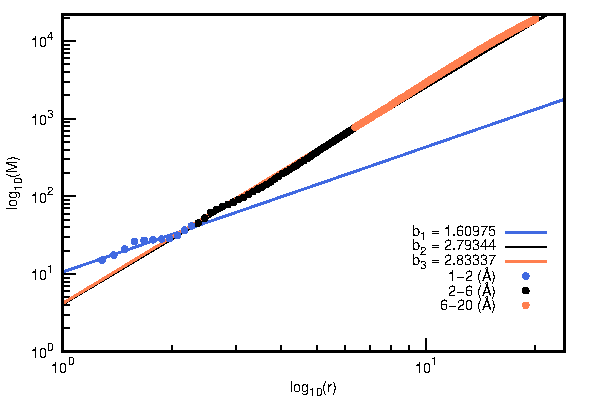
\includegraphics[width=\linewidth,page=1]{graphs/PDBs/1b3e/1b3eEq.pdf}
		\caption{(3)}
	\end{subfigure}
	\hspace{0.2cm}
	\begin{subfigure}{0.49\textwidth} % M\'{a}s ancho para centrar
		\centering
		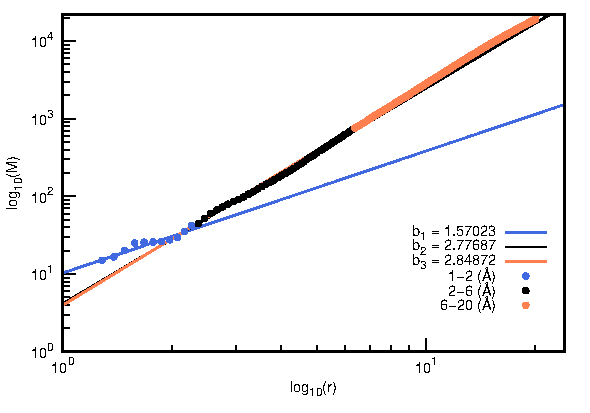
\includegraphics[width=\linewidth,page=1]{graphs/PDBs/1b3e/1b3e1ns.pdf}
		\caption{(4)}
	\end{subfigure}
	\caption{Regresiones lineales de $log_{10}r$ vs $log_{10}M(r)$ correspondiente a cuatro etapas de procesamiento de la s\'{e}ptima prote\'{i}na con \textit{IdPDB:1b3e} de la Tabla \ref{Tabla:ids9}: (1) Adici\'{o}n de \'{a}tomos de hidr\'{o}geno al sistema proteico; (2) al minimizar la energ\'{i´}a de la estructura molecular; (3) equilibrando el sistema bajo condiciones termodin\'{a}micas controladas; y (4) despu\'{e}s de una din\'{a}mica molecular de 1 ns.}
	\label{fig:1b3e}
\end{figure}


\begin{figure}[H]
	\subsection*{IdPDB:7khw}
	
	\hspace{-0.3cm} 
	\begin{subfigure}{0.49\textwidth}
		\centering
		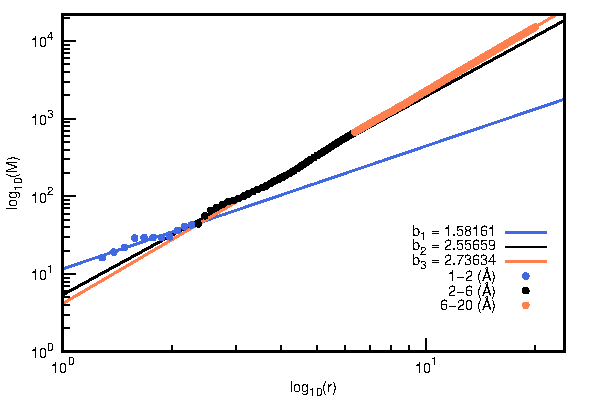
\includegraphics[width=\linewidth,page=1]{graphs/PDBs/7khw/7khwaddH.pdf}
		\caption{(1)}
	\end{subfigure}
	\hspace{0.2cm}
	\begin{subfigure}{0.49\textwidth}
		\centering
		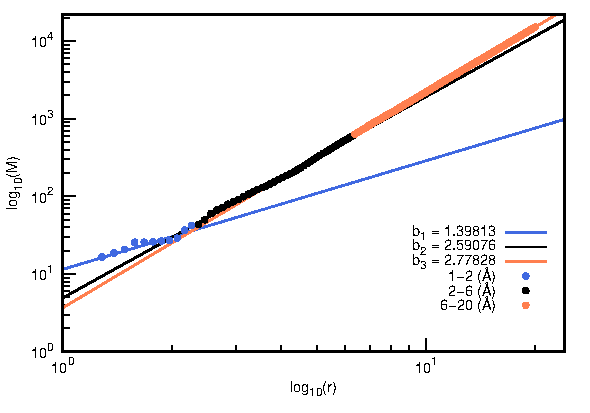
\includegraphics[width=\linewidth,page=1]{graphs/PDBs/7khw/7khwEm.pdf}
		\caption{(2)}
	\end{subfigure}
	
	\vspace{0cm} % Espacio entre filas
	
	\hspace{-0.3cm} 
	\begin{subfigure}{0.49\textwidth}
		\centering
		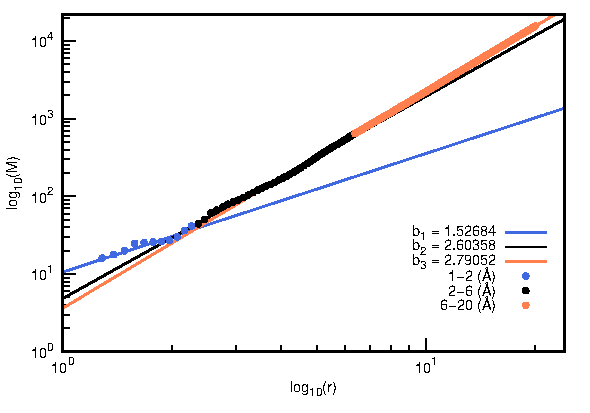
\includegraphics[width=\linewidth,page=1]{graphs/PDBs/7khw/7khwEq.pdf}
		\caption{(3)}
	\end{subfigure}
	\hspace{0.2cm}
	\begin{subfigure}{0.49\textwidth} % M\'{a}s ancho para centrar
		\centering
		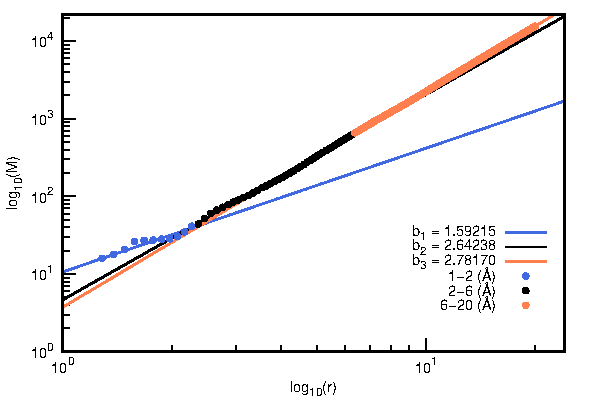
\includegraphics[width=\linewidth,page=1]{graphs/PDBs/7khw/7khw1ns.pdf}
		\caption{(4)}
	\end{subfigure}
	\caption{Regresiones lineales de $log_{10}r$ vs $log_{10}M(r)$ correspondiente a cuatro etapas de procesamiento de la novena prote\'{i}na con \textit{IdPDB:7khw} de la Tabla \ref{Tabla:ids9}: (1) Adici\'{o}n de \'{a}tomos de hidr\'{o}geno al sistema proteico; (2) al minimizar la energ\'{i´}a de la estructura molecular; (3) equilibrando el sistema bajo condiciones termodin\'{a}micas controladas; y (4) despu\'{e}s de una din\'{a}mica molecular de 1 ns.}
	\label{fig:7khw}
\end{figure}

\begin{figure}[H]
	\subsection*{IdPDB:11gs}
	
	\hspace{-0.3cm} 
	\begin{subfigure}{0.49\textwidth}
		\centering
		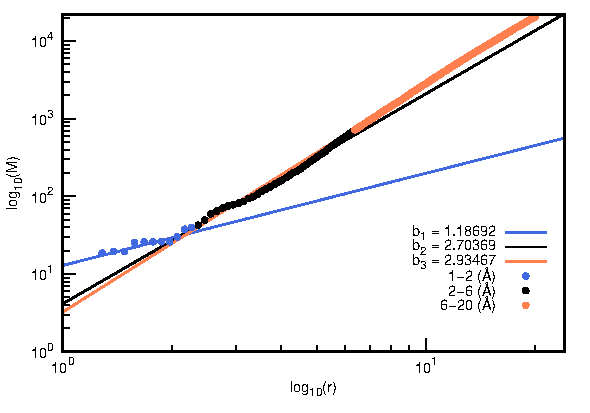
\includegraphics[width=\linewidth,page=1]{graphs/PDBs/11gs/11gsaddH.pdf}
		\caption{(1)}
	\end{subfigure}
	\hspace{0.2cm}
	\begin{subfigure}{0.49\textwidth}
		\centering
		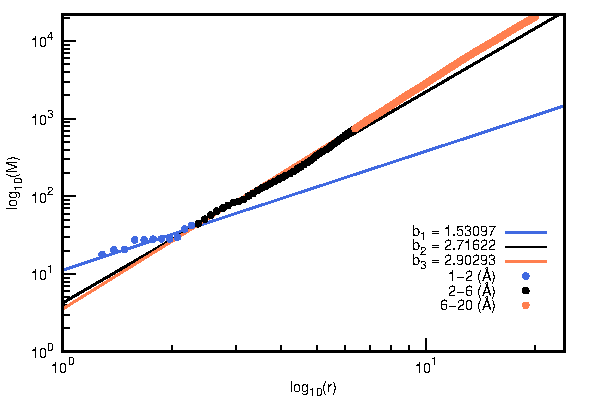
\includegraphics[width=\linewidth,page=1]{graphs/PDBs/11gs/11gsEm.pdf}
		\caption{(2)}
	\end{subfigure}
	
	\vspace{0cm} % Espacio entre filas
	
	\hspace{-0.3cm} 
	\begin{subfigure}{0.49\textwidth}
		\centering
		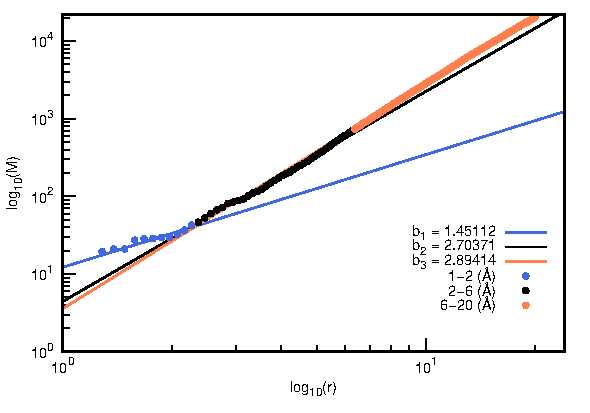
\includegraphics[width=\linewidth,page=1]{graphs/PDBs/11gs/11gsEq.pdf}
		\caption{(3)}
	\end{subfigure}
	\hspace{0.2cm}
	\begin{subfigure}{0.49\textwidth} % M\'{a}s ancho para centrar
		\centering
		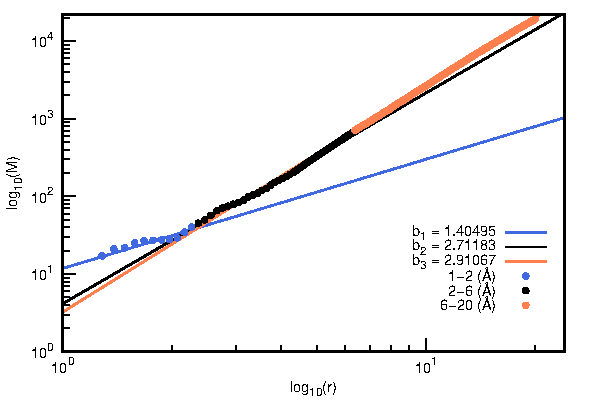
\includegraphics[width=\linewidth,page=1]{graphs/PDBs/11gs/11gs1ns.pdf}
		\caption{(4)}
	\end{subfigure}
	
	\caption{Regresiones lineales de $log_{10}r$ vs $log_{10}M(r)$ correspondiente a cuatro etapas de procesamiento de la octava prote\'{i}na con \textit{IdPDB:11gs} de la Tabla \ref{Tabla:ids9}: (1) Adici\'{o}n de \'{a}tomos de hidr\'{o}geno al sistema proteico; (2) al minimizar la energ\'{i´}a de la estructura molecular; (3) equilibrando el sistema bajo condiciones termodin\'{a}micas controladas; y (4) despu\'{e}s de una din\'{a}mica molecular de 1 ns.}
	\label{fig:11gs}
\end{figure}
´


